
%(BEGIN_QUESTION)
% Copyright 2006, Tony R. Kuphaldt, released under the Creative Commons Attribution License (v 1.0)
% This means you may do almost anything with this work of mine, so long as you give me proper credit

The following hydraulic system is made up of three cylinders connected together by the same tube:

$$\includegraphics[width=15.5cm]{i00152x01.eps}$$

Assuming that all three pistons are the same size, calculate the force generated by the pistons of cylinders \#2 and \#3 if the piston of cylinder \#1 is pushed with 500 pounds of force.

\underbar{file i00152}
%(END_QUESTION)





%(BEGIN_ANSWER)

The force generated at each of the other two pistons will be the same: 500 pounds.  If you were thinking that the 500 applied pound force to cylinder \#1's piston would somehow be divided between the other two pistons, you need to carefully re-consider the pressure/force/area equation.

%(END_ANSWER)





%(BEGIN_NOTES)

What {\it will} be divided between the other two pistons is {\it displacement}.  The combined, linear travel of pistons \#2 and \#3  will equal the travel of cylinder \#1's piston.

\vskip 10pt

If your students are adept at electrical circuit analysis, you might want to use the following analogy to explain the paradox of each cylinder outputting the same force (500 pounds):

$$\includegraphics[width=15.5cm]{i00152x02.eps}$$

Consider this isolation transformer, having three windings with equal turn counts (1000 turns each).  When energized by a 120 volt AC source, the two secondary windings output the same voltage: 120 volts.  Note that the voltage is {\it not} split or divided between the two secondary windings, just as the 500 pound force of the ``master'' piston is not split or divided between the two ``slave'' pistons.

However, {\it current} is definitely divided between the two ``secondary'' windings, just as {\it displacement} is divided between the two slave pistons.  In both systems, the conserved quantity is {\it energy}.  In a lossless transformer, power out ($P_{out} = V_{out} I_{out}$) is equal to power in ($P_{in} = V_{in} I_{in}$).  In a lossless master/slave piston system, work out ($W_{out} = F_{out} \cdot x_{out}$) is equal to work in ($W_{in} = F_{in} \cdot x_{in}$).

%INDEX% Physics, fluids: pressure, force, and area
%INDEX% Physics, static fluids: Pascal's Principle

%(END_NOTES)


